\documentclass{article}
\usepackage[english]{babel}
\usepackage[round,authoryear]{natbib}
\usepackage{graphicx}
\usepackage{amsmath}
\usepackage[most]{tcolorbox}
\usepackage{hyperref}
\bibliographystyle{abbrvnat}

\title{\textbf{MOCCA} \\[0.75cm]
\large An attempt for \\[0.25cm] \textit{a Multi-sourced Ocean Carbonate Chemistry Analysis} \\[2.5cm]
Thesis for the Certificate of Advanced Studies in \textit{Advanced Machine Learning} at University of Bern  \\[2.5cm]
}

\author{Friedrich Anton Burger}
\date{\today}

\begin{document}
	
	\maketitle
	\thispagestyle{empty}
	\vspace{6cm}
	\noindent
	\begin{center}
		Jupyter notebooks with the analyses as well as model parameters can be found in the repository \url{https://github.com/friedrichs-repo/MOCCA/}.
	\end{center}
	
	
	\newpage
	
	\tableofcontents
	\section{Introduction}
	Deep learning has been heavily used in climate science in recent years \citep{reichstein2019}, with applications ranging from forecasting, statistical down-scaling, pattern identification, process parameterization, emulation of physical models, to data interpolation. The success of deep learning in such data-driven applications is based on the versatility of neural networks~\citep{goodfellow2016}. In theory, these can be used to learn any functional relationship between predictors and variables of interest, as reflected by the universal approximation theorem~\cite{hornik1989}.
	
	A particularly important application of deep learning is the interpolation of sparse ship-based measurements of the fugacity of carbon dioxide (fCO$_2$) in the surface ocean. A globally consistent and complete field of fCO$_2$ is necessary to estimate the air-sea CO$_2$ flux and thus necessary to estimate the fraction of anthropogenic carbon emissions that is taken up by the ocean. The global carbon budget \citep{friedlingstein2023}, an annual assessment of global carbon emissions and sinks, currently estimates the oceanic sink from seven observation-based products. While based on very similar underlying fCO2 data and similar mostly satellite-based predictors, these seven products follow different approaches for interpolating the sparse fCO$_2$ data. 
	
	Four of these products are based on feed-forward neural networks: The CMEMS-LSCE-FFNNv2 \citep{chau2022} utilizes a 100-member neural network ensemble,  bootstrapping from the months before and after a fCO$_2$ measurements and leaving the months with fCO$_2$ measurements for independent evaluation. The MPI-SOMFFN \citep{landschuetzer2016} builds on a two step procedure, where first different clusters of similar ocean conditions are determined using a self-organizing map approach and then neural networks are trained to predict fCO$_2$ in each cluster separately. Similarly, OS-ETHZ-GRaCER \citep{gregor2021} provides an ensemble of varying cluster assignments with neural-network-based fCO$_2$ regression in each cluster. NIES-ML3 \citep{zeng2022} is based on three model estimates, from a random forest, a gradient boost machine, and a feed-forward neural network. The remaining three observation-based products build on multiple linear regressions for A$_\text{T}$ and C$_\text{T}$ \citep[fundamental variables to calculate fCO$_2$ and other carbonate system variables; JMA-MLR;][]{iida2021}, extreme gradient boosting to predict the missfit between global ocean biogeochemical models and fCO$_2$ measurements \citep[LDEO-HPD;][]{gloege2022}, and a autoregressive multiple linear regression approach \citep[Jena-MLS;][]{roedenbeck2022}.
	
	The largest uncertainty in these spatially and temporally interpolated fCO$_2$ fields roots in the sparsity and uneven distribution of the underlying fCO$_2$ measurements that are collected in the Surface Ocean CO$_2$ Atlas~\citep{bakker2016}. In particular, measurements are sparse in high-latitude regions and particularly in the Southern Ocean. One approach to soften this issue is applying neural-network based regression seprately in clusters with similar ocean-biogeochemical conditions \citep{landschuetzer2016,gregor2021}, grouping data-sparse regions with others with similar conditions. This project tests another approach to tackle this issue; by not only using fCO$_2$ measurements for training, but also pH measurements from biogeochemical Argo floats~\citep{johnson2017}, which provide critical additional data in the Southern Ocean, and other biogeochemical data as provided by the Global Ocean Data Analysis Project~\citep[GLODAPv2;][]{olsen2016,lauvset2024}. Furthermore, the neural network is here pretrained on CMIP6 Earth system models to test whether this fosters inference of surface fCO$_2$ in sparsely sampled ocean regions with the prior knowledge about functional relationships from Earth system models. The use of multiple sources of data is enabled by a flexible model structure that allows to train on multiple target variables. Similarly to \cite{iida2021}, the approach taken here could, in theory, provide coherent estimates for all variables of the oceanic carbonate system. However, facing problems with sparseness of non-fCO$_2$ data and limited transferability of the functional relationships from climate models to real world data, the approach taken does not improve spatial interpolation of surface-ocean fCO$_2$.
	
	\section{Overall model architecture}
	\begin{figure}
		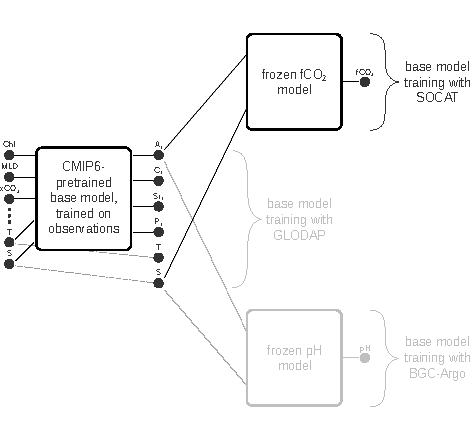
\includegraphics[width=0.85\textwidth]{./figures/model_architecture_greyed_out_parts.pdf}
		\caption{Scheme displaying the overall planned model architecture for MOCCA. Components in grey colors will eventually not be used due to insufficient data availability from GLODAP and BGC-Argo.}
		\label{fig:fco2_model}
	\end{figure}
	The model architecture, here called \textit{MOCCA} for brevity, is based on a three-step procedure~(Figure~\ref{fig:fco2_model}): \\
	
	\underline{$\mathbf{1}$} \hspace{0.2cm} In a first step (section \ref{sect:surrgate_models}), surrogate neural network models are trained to fit the functional relationship between a set of variables needed to solve the oceanic carbonate system (\textit{carbonate chemistry drivers}) and two specific carbonate chemistry variables, pH and fugacity of CO$_2$ (Section~\ref{sect:surrgate_models}). The functional relationship is learned from the numerical carbonate chemistry package \textit{mocsy 2.0} \citep{orr2015}. Using the numerical carbonate chemistry package directly in the neural network training would consume too much time and is thus not feasible. This step is performed first to identify appropriate hyper parameters and training procedure in a situation where near-perfect learning is possible. \\
	
	\underline{$\mathbf{2}$}\hspace{0.2cm} In a second step (section \ref{sect:cmip6-pretraining}), a neural network is trained on model output from CMIP6 Earth system models to learn the statistical relationships between a set of predictors and the carbonate chemistry drivers. This model will serve as a prior estimate to improve inference for fCO$_2$ and pH in undersampled regions where only few fCO$_2$ and pH measurements are available. \\
	
	\underline{$\mathbf{3}$}\hspace{0.2cm} In a third step (section \ref{sect:obs-tuning}), the CMIP6-pretrained base model from the previous step is trained with observational data for fCO$_2$ from the Surface Ocean CO$_2$ Atlas (SOCAT). To do so, the surrogate fCO$_2$ neural network (frozen to prevent parameter updates) is combined with the pretrained base model, and the loss is calculated between predicted fCO$_2$ and SOCAT data. The original idea was to also include carbonate chemistry drivers from GLODAP, and pH from BGC-Argo floats, with the loss is either directly calculated from the output of the base model (GLODAP), or from the output of the surrogate fCO$_2$ or pH models (for SOCAT and BGC-Argo respectively). However, it will be seen that inclusion of GLODAP and BGC-Argo data, as envisioned here, is not feasible.
	
	, 
	
	\section{Surrogate models for mocsy fCO2 and pH} \label{sect:surrgate_models}
	\begin{tcolorbox}[colback=gray!5!white, colframe=black!75!white, 
		fonttitle=\bfseries, title=Jupyter Notebooks, 
		rounded corners, width=\textwidth]
		train\_fco2\_model.ipynb \\
		train\_ph\_model.ipynb
	\end{tcolorbox}
	In a first step, surrogate multi-layer perceptron models were trained to replace numerical solution of the oceanic carbonate system. To do so, samples for total alkalinity (A$_\textup{T}$), dissolved inorganic carbon (C$_\textup{T}$), temperature (T),  salinity (S), total silicate (Si$_\textup{T}$), and total phosphate (P$_\textup{T}$) were randomly generated from uniform distributions (Table~\ref{tab:gen_data}). \\
	The training data size was set to 5 000 000 samples and the validation data size was set to 1 000 000 samples. Mocsy 2.0 (Orr et al., 2015a) was then used to calculate fCO$_2$ and pH for these samples. After normalizing per feature with the means and standard deviations given in Table~\ref{tab:gen_data}, multilayer perceptron models with three identical hidden layers were trained with mocsy fCO$_2$ and pH as labels. \\
	For fCO$_2$, model complexity was iteratively increased until a desired maximum deviation of less than 1\,$\mu$atm was reached (the measurement uncertainty for pCO$_2$ as reported by Orr et al, 2015b)\footnote{For reference, fCO$_2$ across the generated samples varies between 0.001\,$\mu$atm and 5108\,$\mu$atm.}. During training, learning rate was decreased from 10$^{-3}$ to 10$^{-5}$ following an exponential learning rate schedule over 10 000 epochs. The decay in learning rate was chosen to shift from an initial identification of an optimal region in the parameter space to finding an optimal set of parameters for which the mean squared error over the training and validation sets converges to a similar and low value. \\
	Hidden layer size was increased from an initial 64 hidden layer units (8833 trainable parameters), 80 units (13601 parameters), 96 units (19393 parameters), 128 units (34049 parameters), to 160 units (52801 parameters). The largest model\footnote{To give some context about the model complexity: The number of paramters of this model is comparable to that of a Taylor expansion of a function with six arguments to 15th order. Assuming an efficient use of the MLP parameters, a good fit to the numerical solution from mocsy is thus expected.} hit a maximum deviation of 1.08\,$\mu$atm over the validation set (Figure~\ref{fig:surrogate_model_accuracy}).
	The same model architecture was then also used to train the pH model, resulting in a maximum deviation over the validation set of 0.0044. \\
	With root mean squared errors (RMSE) of 0.026\,$\mu$atm (fCO$_2$ model) and 0.00008 (pH model), these surrogate models provide a precision that is comparable to numerical carbonate chemistry packages: Orr et al., 2015b report a desired numerical uncertainty of 0.1\,$\mu$atm and 0.0003, respectively. \\
	The accurracy of the fCO$_2$ and pH neural network models is similar for the six million random samples for A$_\text{T}$, C$_\text{T}$, T, S, Si$_\text{T}$, and P$_\text{T}$ from the CMIP6 models (section~\ref{sect:cmip6-pretraining}). Specifically, RMSE is 0.029\,$\mu$atm and 0.00006, respectively, and the maximum deviations are 0.24\,$\mu$atm and 0.0006, respectively.     
	
	\begin{table}
		\centering
		\bgroup
		\def\arraystretch{1.5}
		\begin{tabular}{c|c|c}
			& minimum & maximum \\
			\hline 
			A$_\textup{T}$ & 1000\,$\mu$mol\,kg$^{-1}$ & 3000\,$\mu$mol\,kg$^{-1}$ \\
			\hline
			C$_\textup{T}$ & 1000\,$\mu$mol\,kg$^{-1}$ & A$_\textup{T}$ \\
			\hline
			T & -2\,°C & 35\,°C \\
			\hline
			S & 10\,PSU & 50\,PSU \\
			\hline
			Si$_\textup{T}$ & 0\,$\mu$mol\,kg$^{-1}$ & 134\,$\mu$mol\,kg$^{-1}$ \\
			\hline
			P$_\textup{T}$ & 0\,$\mu$mol\,kg$^{-1}$ & 4\,$\mu$mol\,kg$^{-1}$ \\
			
		\end{tabular}
		\egroup
		\caption{Minima and maxima of the uniform distributions used to generate samples for the fCO$_2$ and pH surrogate models. The range for A$_\textup{T}$ was chosen such that it easily encompasses open ocean variations in A$_\textup{T}$. That for C$_\textup{T}$ is limited to values lower A$_\textup{T}$ since larger C$_\textup{T}$ do not occur in the ocean. The ranges for T and S are chosen according to Lueker et al., 2000, whose parameterizations for K$_1$ and K$_2$ are used in mocsy. Finally, the maximum values for Si$_\textup{T}$ and P$_\textup{T}$ were chosen to be the global maxima found in the monthly climatologies for Si$_\textup{T}$ and P$_\textup{T}$ from World Ocean Atlas 2023. These uniform distributions have means $(max + min) / 2$ and standard deviations $(max - min) / \sqrt{12}$, expcept for C$_\textup{T}$ where mean and standard deviation are given by $min + (max - min) / 4$ and $(max - min) \cdot \sqrt{7 / 144}$, respectively. These means and standard deviations are used for feature normalization.}
		\label{tab:gen_data}
	\end{table}
	\begin{figure}
		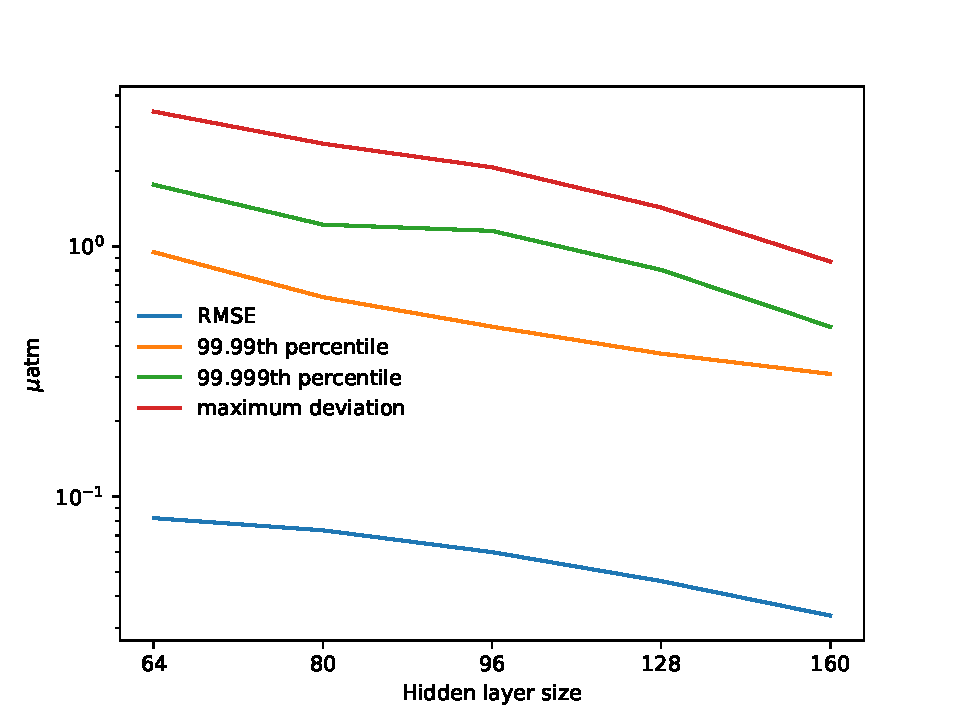
\includegraphics[width=0.85\textwidth]{./figures/fco2_model_error_vs_hidden_layer_size.pdf}
		\caption{The evolution of root mean squared error (RMSE), the 99.99th and 99.999th percentiles of deviation and the maximum deviation between the surrogate model and mocsy fCO$_2$ over the validation data set with 1000 000 randomly generated samples.}
		\label{fig:surrogate_model_accuracy}
	\end{figure}
	\section{CMIP6-pretrained base model} \label{sect:cmip6-pretraining}
	\begin{tcolorbox}[colback=gray!5!white, colframe=black!75!white, 
		fonttitle=\bfseries, title=Jupyter Notebooks, 
		rounded corners, width=\textwidth]
		CMIP6\_data\_preparation.ipynb \\
		train\_CMIP6\_base\_model.ipynb \\
		\textbf{under ./single\_CMIP6\_model\_experiments:} \\
		CMIP6\_data\_preparation\_1model.ipynb \\
		train\_CMIP6\_base\_model\_1model.ipynb \\
		train\_CMIP6\_base\_model\_1model\_with\_cld\_pr.ipynb \\
		train\_CMIP6\_base\_model\_1model\_large\_model.ipynb
	\end{tcolorbox}

	As a first step, we pre-train a neural network on the statistical relationships between predictor variables and sea surface A$_\textup{T}$, C$_\textup{T}$, Si$_\textup{T}$, and P$_\textup{T}$. The predictor variables chosen here are sea surface temperature (SST), sea surface salinity (SSS), mixed layer depth (MLD), sea surface height (SSH), chlorophyll-a concentration (chl), sea ice concentration (ice), 10\,m easterly wind (u), 10\,m northerly wind (v),
	% precipitation (pr), cloud cover (cld),
	dry volume molar ratio of CO$_2$ in the atmosphere (CO$_2$), sinus and cosinus of the month of year ($\sin(m / 12 \cdot 2\pi)$ and $cos(m / 12 \cdot 2\pi)$), as well as latitude and longitude encoded using spherical coordinates following \cite{gade2010}. The representations for month of year and location are used to avoid discontinuities in the months between December and January and in longitude at the dateline ($\pm180$\,°E).
	
	The neural network is trained on 6 million samples (5 million for training and 1 million for validation) that were evenly drawn from three CMIP6 Earth system models: the UKESM1-0-LL, the MPI-ESM1-2-LR, and the CMCC-ESM2. Despite a high-resolution version of the MPI model, these were the only ones to provide all predictors on monthly-mean resolution. Data from multiple Earth system models were used to ensure that the model learns general relationships that are not specific to a certain Earth system model with respective biases. The model data is taken from the period 1993-2022 (\textit{historical} simulation until 2014, followed by \textit{SSP2-4.5}). The predictors MLD and chl were log-transformed prior to training to foster learning. The log transformation was applied only where the resulting distribution was more Gaussian (where the test statistic of a Kolmogorov-Smirnov test, i.e. the maximum difference between the empirical distribution function of the data and the distribution function of a standard normal distribution, was smaller after transformation). 
	Finally the predictors for the CMIP6 pre-trained base model are nromalized to zero mean and unit variance and the 4 labels are normalized as specified in Table~\ref{tab:gen_data} (to match the normalization used for the fCO$_2$ and pH surrogate models).
	
	For the training, the same architecture that was already used to train the surrogate models (despite not applying a final ELU non-linearity on the output layer, such that the last hidden layer is linearly projected) is used, again with 10\,000 epochs and a batch size of 1000. Root mean squared errors of 6.1\,$\mu$mol\,kg$^{-1}$ (A$_\textup{T}$), 6.3\,$\mu$mol\,kg$^{-1}$ (C$_\textup{T}$), 0.8\,$\mu$mol\,kg$^{-1}$ (Si$_\textup{T}$), and 0.03\,$\mu$mol\,kg$^{-1}$ (P$_\textup{T}$) are obtained (on the validation set and after backtransforming to unnormalized labels). As such, RMSEs are more than a magnitude lower than the standard deviations of A$_\textup{T}$, C$_\textup{T}$, Si$_\textup{T}$, and P$_\textup{T}$ in the CMIP6 model data samples, given by 111.7, 99.1, 26.3, and 0.5\,$\mu$mol\,kg$^{-1}$, respectively\footnote{RMSE equals the standard deviation for a model that always predicts the mean of a variable. Hence, a lower RMSE implies skill in predicting spatial and temporal variations in the variable (also see the discussion on the fraction of variance unexplained in section~\ref{sect:obs-tuning}).}. Likely owing to the large size of the training data set relative to the model complexity and  to the consistency of the climate model data, overfitting appears not to be a problem. The validation loss continuously decreases, ending up 11\,\% larger than the training loss\footnote{Technically speaking, the training data loss is calculated for all batches in an epoch separately and then averaged. It is thus calculated slightly different than the validation loss.}.
	
	A part of this error can be explained by the fact that the neural network mapping is necessarily imperfect since the three models imply different statistical relationships between predictors and labels. Creating 6 million samples only from the UKESM1-0-LL model, the root mean squared errors become significantly smaller, now being 4.0\,$\mu$mol\,kg$^{-1}$ for A$_\textup{T}$, 4.2\,$\mu$mol\,kg$^{-1}$ for C$_\textup{T}$, 0.5\,$\mu$mol\,kg$^{-1}$ for Si$_\textup{T}$, and 0.02\,$\mu$mol\,kg$^{-1}$ for P$_\textup{T}$. The remaining errors should be mainly due to insufficient information in the predictor variables to fully explain the variations in the four concentrations. Adding further predictors may enhance the skill of a model. However, an experiment with total cloud cover and precipitaion as additional atmospheric predictors resulted only in marginal improvements of errors. In another sensitivity test, the training using UKESM1-0-LL model data was also repeated using a much wider model architecture (256 units per hidden layer, 150\,\% increase in number of parameters). In the first half of the training, validation loss steadily declines, becoming 24\,\% smaller than the validation loss for the default model architecture with 160 units per hidden layer. This highlights a potential for increasing model performance with a larger neural network to a certain extent. In the second half of the training, however, overfitting results in a steady increase in validation loss. As such, a fully-connected neural network of this size requires either more training data to converge without overfitting or some regularization technique. Given that there is an order of magnitude less data availble from observations, the smaller network architecture appears to be a good choice for the next step, where the model is fine-tuned with observational data following a transfer learning protocol. 
	
	\section{Model tuning on observational data} \label{sect:obs-tuning}
	\begin{tcolorbox}[colback=gray!5!white, colframe=black!75!white, 
	fonttitle=\bfseries, title=Jupyter Notebooks, 
	rounded corners, width=\textwidth]
	gridding\_the\_GLODAP\_data.ipynb \\
	gridding\_the\_bgc-argo\_data.ipynb \\
	consistency\_of\_GLODAP\_with\_BGC-Argo\_and\_SOCAT.ipynb \\
	train\_base\_model\_on\_SOCAT.ipynb \\
	training\_on\_SOCAT\_varying\_complexity\_and\_dropout.ipynb \\
	\textbf{under ./single\_CMIP6\_model\_experiments:} \\
	train\_base\_model\_1model\_on\_MPI\_ESM.ipynb
	\end{tcolorbox}
	\subsection{Observational data preparation}
	In this step, the CMIP6-pretrained base model shall be trained on observational data. The data products used for each predictor are listed in Table\,\ref{tab:pred_data} and those intended to be used as label data are listed in Table\,\ref{tab:label_data}. The predictor data are generally on much higher-resolution than the regular 1°-latitude $\times$ 1°-longitude grid used here. As such the data for SST, SSS, MLD, chl, ice, SSH, u, and v were first binned to this coarser resolution. For CO$_2$, a global and annual-average representative value was used. The Surface Ocean CO$_2$ Atlas (SOCAT) provides average fCO$_2$ measurements on the desired 1°$\times$1° grid. The data from GLODAP and BGC-Argo, however is only available as individual ungridded measurements. These data are here gridded first (see jupyter notebooks listed above). From GLODAP, two different types of gridded data are derived; one with all four concentrations (A$_\text{T}$, C$_\text{T}$, Si$_\text{T}$, and P$_\text{T}$) available, and one only with A$_\text{T}$ and C$_\text{T}$ (the more important quantities) available. As a result, four data categories are created for training and validation: SOCAT, BGC-Argo, GLODAP-4, and GLODAP-2. Removing grid values where not all predictors provide data, these data categories encompass 324296, 9449, 10629, and 3959 gridded values, respectively. 
	
	\begin{table}
		\centering
		\bgroup
		\def\arraystretch{1.5}
		\begin{tabular}{c|c}
			Predictor & Data product \\ \hline
			Sea surface temperature & ESA SST CCI and C3S$^1$  \\
			Sea ice fraction & ESA SST CCI and C3S$^1$  \\
			Sea surface salinity & CMEMS ARMOR3D L4$^2$ \\
			Mixed layer depth & CMEMS ARMOR3D L4$^2$ \\
			Sea surface height & CMEMS L4 Sea Surface Heights$^3$ \\
			Chlorophyll-a concentration & Copernicus-GlobColour$^4$ \\
			CO$_2$ mole fraction & Manua Loa Hawaii in-situ data$^5$ \\ %CAMS CO2 atmospheric inversion$^5$
			Eastward near-surface wind & ECMWF Reanalysis v5 (ERA5)$^6$ \\
			Northward near-surface wind & ECMWF Reanalysis v5 (ERA5)$^6$
		\end{tabular}
		\egroup
		\caption{List of predictors used to predict A$_\textup{T}$, C$_\textup{T}$, Si$_\textup{T}$, and P$_\textup{T}$ and the data product used for each predictor. $^1$\url{https://doi.org/10.48670/moi-00169}; only available until Oct. 2022, $^2$\url{https://doi.org/10.48670/moi-00052}, $^3$\url{https://doi.org/10.48670/moi-00148},
			$^4$\url{https://doi.org/10.48670/moi-00281}; only available from Sept. 1997 on, $^5$\url{https://scrippsco2.ucsd.edu/data/atmospheric_co2/primary_mlo_co2_record.html}, 
			$^6$\url{https://cds.climate.copernicus.eu/cdsapp\#!/dataset/reanalysis-era5-single-levels-monthly-means}}
		\label{tab:pred_data}
	\end{table}
	
	\begin{table}
		\centering
		\bgroup
		\def\arraystretch{1.5}
		\begin{tabular}{c|c}
			Label & Data product \\ \hline
			fCO2 & SOCATv2023$^1$ \\
			A$_\text{T}$, C$_\text{T}$, Si$_\text{T}$, P$_\text{T}$ & GLODAPv2 2023$^2$ \\
			pH & BGC-Argo$^3$
		\end{tabular}
		\egroup
		\caption{List of label data used to train the base model. $^1$\url{https://socat.info/index.php/2023/06/20/v2023-release/}, $^2$\url{https://glodap.info/index.php/merged-and-adjusted-data-product-v2-2023/}, $^3$\url{https://www.seanoe.org/data/00311/42182/}}
		\label{tab:label_data}
	\end{table}
	
	Given the small amount of data available from GLODAP and BGC-Argo, only few data are used to calculate the grid cell values. For example for GLODAP-4, 60\% of grid cells are just representing one measurement, 88\% of cells represent the average of maximally two measurements. This is in contrast to SOCAT, where the percentage of grid cells based on one or maximally two measurements is 3\% and 6\%, respectively. It is therefore questionable whether these derived gridded fields adequately represent the mean conditions in the grid cells, which extend over an area of about a 100\,km$\times$100\,km and over a month. To test the adequacy of representation, the three data-sets are cross-compared in overlapping grid cells (Figure~\ref{fig:cross-comparison}). As a baseline, pH is calculated from GLODAP-4 data and compared to the pH measurements provided by GLODAP (Figure~\ref{fig:cross-comparison}a), providing information about the effect of measurement uncertainty and uncertainty in the carbonate chemistry calculation. The root mean squared error of 0.006 is smaller than the estimated measurement uncertainty of pH of 0.01~\cite{lauvset2024}. As such, almost all variance in the calculated pH can be explained by the pH measurements (ratio of mean squared error to variance in calculated pH (the fraction of unexplained variance) is only 3\,\%). In contrast, BGC-Argo derived pH has much less explanatory power (Figure~\ref{fig:cross-comparison}b), with 63\,\% of the variance in calculated GLODAP pH unexplained. With the only difference between panels a) and b) being the additional uncertainty from the poor representation of grid values from few measurements, this step seems to crucially reduce the quality of the data. Similarly, large discrepancies are also found when comparing GLODAP-calculated fCO$_2$ with SOCAT fCO$_2$ measurements (Figure~\ref{fig:cross-comparison}c), with a root mean squared error of 34\,$\mu$atm. Overall, I here conclude that the quality of the gridded fields derived from GLODAP and BGC-Argo is not sufficient for them to be used as additional sources to train a neural network alongside the more robust SOCAT data.
	
	\begin{figure}
		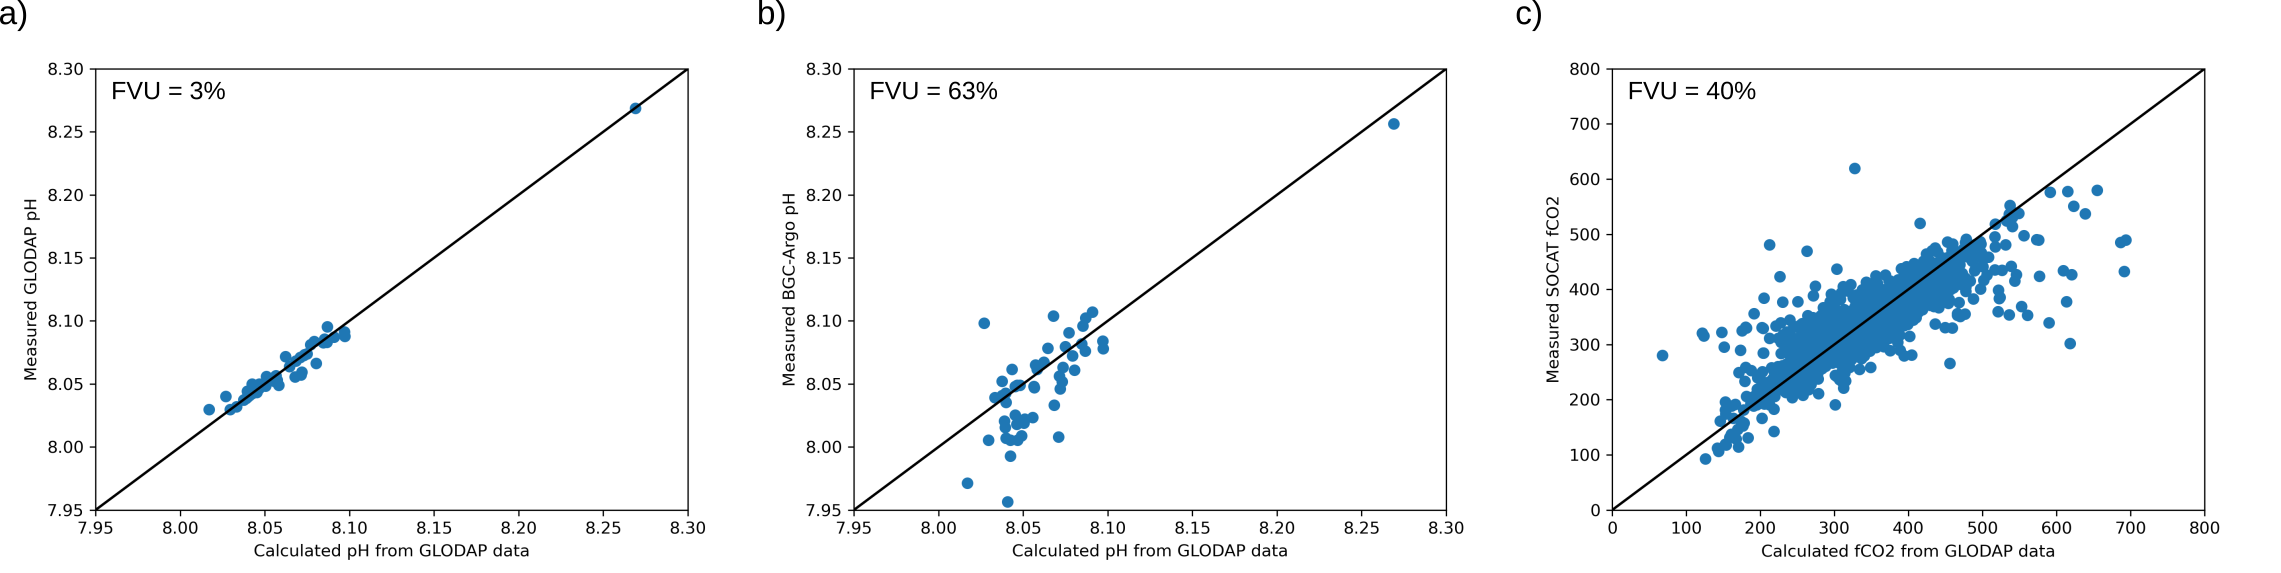
\includegraphics[width=\textwidth]{./figures/consistency_GLODAP-bgc-argo_SOCAT.png}
		\caption{Cross-comparison of data from the gridded GLODAP-4, BGC-Argo, and SOCAT fields where overlapping. (a,b) Comparison of pH calculated from GLODAP-4 variables to measured pH from GLODAP (a) and from BGC-Argo (b). Both panels only show data for grid cells where data from GLODAP and BGC-Argo is available. (c) Comparison  of fCO$_2$ calculated from GLODAP-4 to measured fCO$_2$ from SOCAT. The fraction of variance unexplained (FVU) is given in each panel. FVU is the ratio of the mean squared error (MSE) to the variance of the explained variable. An FVU of 0\% indicates a perfect representation, while an FVU of 100\% indicates that no variations can be explained, corresponding to a model that always predicts the mean (in which case MSE equals variance).
		}
		\label{fig:cross-comparison}
	\end{figure}
	
	\subsection{Test case: tuning a CMIP6 pre-trained model on data from another model}
	\label{subsection:cmip6training}
	After having established to only use SOCAT observational data, we now proceed with fine-tuning the CMIP6-pretrained base model on the SOCAT data. The fine-tuning approach is motivated by the relatively low amount of observational data compared to neural network complexity and by the biased distribution of observational data. In contrast, climate model data is abundant and available everywhere in the world ocean. As such, a neural network pretrained on climate model data may be less spatially biased. The fine-tuning roughly follow the protocol by \cite{geron2019hands}, who proposes to first retrain the final layer of the model (the last linear projection layer of the base model in this case), and then to subsequently unfreeze more layers, proceeding from the output side to the input side of the network, and to fine-tune them with a small learning rate, until model performance on the validation data does not improve anymore. \\
	
	The procedure is here first tested in a controlled environment: The pretrained model based on data from the UKESM model only (introduced in section \ref{sect:cmip6-pretraining}) is here tuned with fCO$_2$ labels and the set of 14 predictors (incl. representations of month of year and geographical location as outlined in section \ref{sect:cmip6-pretraining}) from the MPI model. To archieve a comparable situation to real data, the data is constrained to where also SOCAT data is available, resuling in 305636 samples. The 14 predictors are normalized with the means and standard deviations from the UKESM samples. This is done to improve 'out-of-the-box' UKESM-pretrained model performance on the MPI-ESM data. Following the scheme in Fig.\,\ref{fig:fco2_model}, a modular MLP is then defined, with the base model with pretrained weights and biases from UKESM data, and the frozen surrogate fCO2 model mapping the output from the base model to fCO$_2$ if a respective flag is provided in the MLP model call. \\
	
	First, the \textit{zero-shot} regression performance is tested. The mean squared error exceeds variance on the validation set (RMSE of 53\,$\mu$atm), indicating near-zero predictive skill for fCO$_2$ based on the pre-training on another climate model. Retraining the last projection layer of the base model drastically increases model skill, resulting in a RMSE of 17\,$\mu$atm and a fraction of variance unexplained (FVU) of only 16\%. Retraining the second-last layer with a low learning rate (decaying from 10$^{-4}$ to 10$^{-5}$), and subsequently finetuning the whole base model with a learning rate of 10$^{-5}$, RMSE drops to 5.7\,$\mu$atm and FVU to 1.7\,\%. \\
	
	However, as already indicated by the poor \textit{zero-shot} performance, there is no advantage from tuning a base model that was pre-trained with spatially uniformly distributed data from another climate model, at least when testing performance on the necessarily also spatially biased validation set: When training a neural network from scratch on the MPI model, RMSE is 5.2\,$\mu$atm and FVU to 1.4\,\%. As such, almost all variations in fCO$_2$ in the validation set can be resolved based on the 14 predictors, irrespective of fine-tuning or training from scratch. It can thus also be concluded that the predictors contain sufficient information to resolve almost all variations in fCO$_2$, and that, despite the small sample size compared to model complexity, overfitting is not problematic for the case of climate model data. \\
	
	Since training neural networks here on climate model data, one can also analyse RMSE on the whole grid - allowing to see how the trained neural networks perform in data-sparse regions (Figure ~\ref{fig:global-rmse}). The comparison of the two models on the complete global data again shows no advantage of the pretrained model over that trained from scratch. On the contrary, the latter model performs better in data-sparse high-latitude regions. Furthermore, it consistently shows a much lower RMSE compared to temporal standard deviation of fCO$_2$ except in the Arctic Ocean (north of 70\,°N), indicating capability of resolving spatial and temporal variations in fCO$_2$ outside well-sampled regions.  \\
	
	\begin{figure}
	\centering
	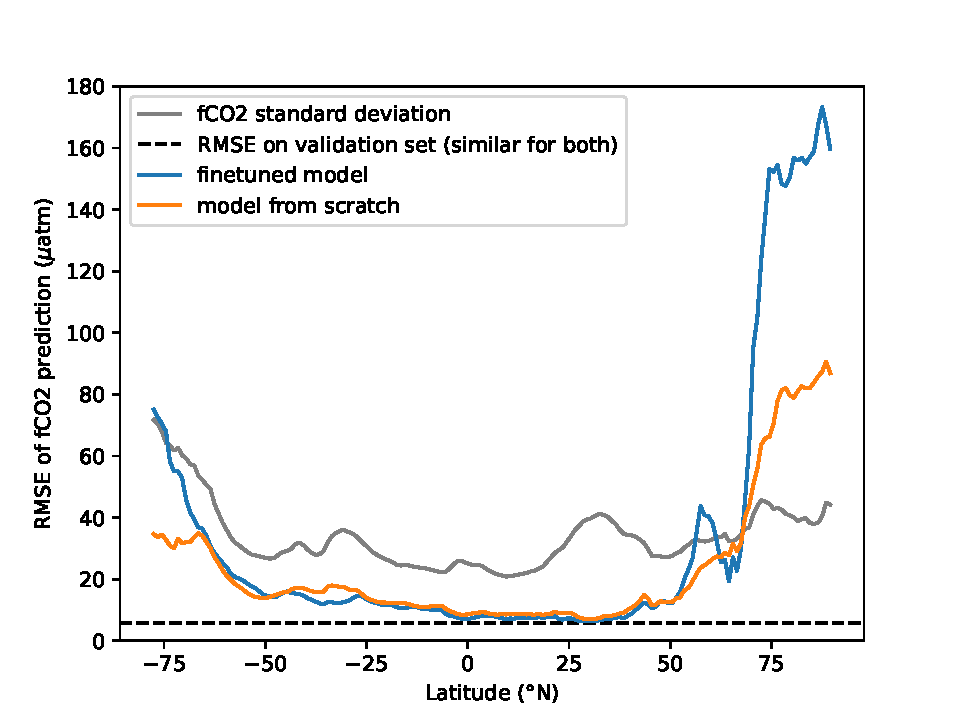
\includegraphics[width=0.75\textwidth]{./figures/MPI-ESM_global_model_rmse.pdf}
	\caption{Zonal mean of the root mean squared error (RMSE) in each grid cell over the full 30 year period, calculated between simulated fCO$_2$ and fCO$_2$ predicted by the fine-tuned neural network and the neural network trained from scratch on data from the MPI model. The grey dashed line indicates the RMSE on the spatially biased validation set (similar for both models). The grey line shows the zonal mean temporal standard deviation of simulated fCO2. The ratio between RMSE and standard deviation (the square root of FVU) indicates how much temporal variability can be resolved by predicted fCO$_2$.}
	\label{fig:global-rmse}
	\end{figure} 
	
	Finally, it is interesting to see what kind of solutions for A$_\textup{T}$, C$_\textup{T}$, Si$_\textup{T}$, and P$_\textup{T}$ are predicted after training on fCO$_2$. The mapping $(\textup{A}_\textup{T}, \textup{C}_\textup{T}, \textup{Si}_\textup{T}, \textup{P}_\textup{T}) \rightarrow \textup{fCO}_2$ is no bijection, different combinations of input variables can result in the same fCO$_2$, e.g. through an infinitesimal change in the input variables that satisfies $\Sigma_i \partial \textup{fCO} / \partial x_i \cdot \delta x_i = 0$. As a result, the neural network finds solutions for A$_\textup{T}$, C$_\textup{T}$, Si$_\textup{T}$, and P$_\textup{T}$ that predict a correct fCO$_2$, but are far off realistic values. Specifically, the trained network predicts too large values for all four variables (see notebook train\_base\_model\_1model\_on\_MPI\_ESM). As a result, the predicted solution for the four variables can not be expected to yield a realistic result for other carbonate chemistry variables such as pH. This limitation could be potentially overcome by finding a way to include training data for pH (BGC-Argo) and  A$_\textup{T}$, C$_\textup{T}$, Si$_\textup{T}$, and P$_\textup{T}$ (GLODAP).
	
	
	\subsection{Training on SOCAT data}
	
	The fine tuning procedure is now applied to real observational data (notebook train\_base\_model\_on\_SOCAT.ipynb). The total sample size, i.e. grid cells where data from all predictors as well as SOCAT fCO$_2$ label data is available, is given by 311440. The 14 predictors from real world data are normalized with the means and standard deviations from the CMIP6 samples, again to improve \textit{out-of-the-box} CMIP6-pretrained model performance on the observational data. The modular MLP model is defined as introduced in subsection \ref{subsection:cmip6training}, but with weights and biases from the base model pretrained on all three CMIP6 models. \\
	
	
	As a first experiment, the CMIP6-pretrained model is used to predict fCO$_2$ without prior training on the observational data. In this zero-shot inference scenario, the model predicts fCO$_2$ with a RMSE of 35\,$\mu$atm on the validation set. As such it can not resolve most of the variance in the fCO$_2$ validation set (FVU of 73\,\%), highlighting limited predictive power without training on observational data.  \\
	
	In a next step, the base-model should be finetuned on observational data, as it was done on the MPI Earth system model in subsection \ref{subsection:cmip6training}. As for the case of transfer learning with Earth system model data, retraining the last projection layer of the base model clearly increases model skill, resulting in a RMSE of 26\,$\mu$atm and a fraction of variance unexplained (FVU) of only 39\%. Retraining the second-last layer with a low learning rate (decaying from 10$^{-4}$ to 10$^{-5}$), RMSE becomes 19\,$\mu$atm with a FVU of 20\,\%. \\
	
	As for the Earth system model data case, finetuning a CMIP6-pretrained model is not improving loss on the validation set compared to training a model from scratch on SOCAT data only. In the latter case, RMSE after training is 18\,$\mu$atm. As such, fine-tuning a CMIP-pretrained model does not improve accuracy on unseen data compared to training a model from scratch. In contrast to the Earth system model data only case, however, overfitting is observed: the validation loss approaches 16\,$\mu$atm early in the training, followed by a degradation of performance on the validation set. \\
	
	With no advantage of using the pretrained model proposing to train a model from scratch, the question of an optimal architecture for such a model, providing sufficient complexity for a global regression of fCO$_2$ while avoiding overfitting, remains. In the following, three smaller networks, and two with regularization achieved by dropout layers~\citep{srivastava20124dropout} are tested (notebook training\_on\_SOCAT\_varying\_complexity\_and\_dropout.ipynb). To simplify training, these neural networks predict fCO$_2$ directly, given that there is no advantage of predicting A$_\text{T}$, C$_\text{T}$, Si$_\text{T}$, and P$_\text{T}$ in the absence of GLODAP and BGC-Argo training data. Furthermore, the predictor data is now directly normalized based on the training data set, since there is no use of normalizing the predictors to CMIP6 means and standard deviations when not starting from a CMIP6-pretrained model. This should improve learning during training.   \\
	
	The three smaller networks are chosen such that the number of parameters increases by a factor of 4 between each, from 801 parameters (three hidden layers of size 16) to 3241 parameters (hidden layer size 36) to 12921 parameters (hidden layer size of 76) to 54081 parameters (the default neural network used before; hidden layer size of 160).  The methodology for dropout follows \cite{srivastava2014}, using dropout layers between the three hidden layers, a dropout rate of 20\,\%, and a high initial learning rate of 10$^{-2}$. Hidden layer size is chosen as 160 (default) and 324 (215785 parameters). \\ 
	
	
	\begin{figure}
		\centering
		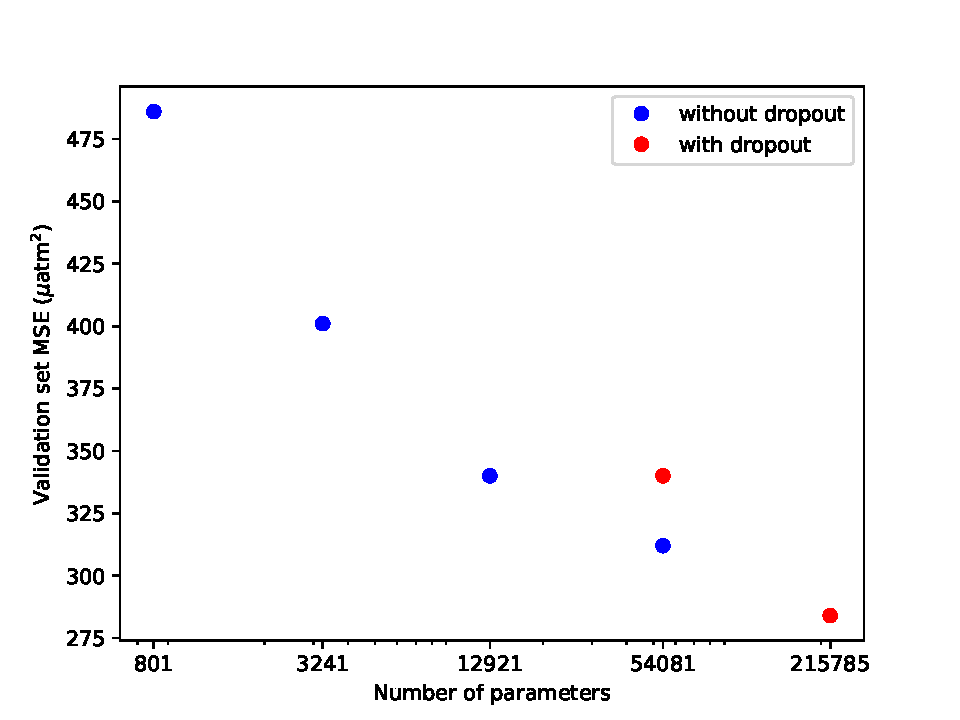
\includegraphics[width=0.75\textwidth]{./figures/fco2_training_on_obs_complexity_and_dropout.pdf}
		\caption{Validation loss (MSE) for training on observed fCO$_2$ from SOCAT as a function of model complexity (number of parameters). Blue dots indicate networks without dropout layers and red dots indicate networks with dropout.}
		\label{fig:mse_vs_complexity}
	\end{figure}
	
	 With increasing model complexity, loss on the validation set generally decreases(Figure~\ref{fig:mse_vs_complexity}). For the smaller neural networks overfitting does not occur, as indicated by a steady decline of validation loss during training and by comparable loss on the training and validation sets. With overfitting present for the default network size (54081 parameters), dropout offers a means of further increasing model complexity while avoiding a loss of generalizability. As discussed in \cite{srivastava2014}, networks with dropout require larger hidden layers for the same network performance. As such, it comes as no surprise that a model without dropout at 54081 parameters performs better on the validation set than one with dropout (Figure~\ref{fig:mse_vs_complexity}). However, the large model with dropout (215785 parameters) performs superior, and, at the same time, shows no sign of overfitting (validation and training loss comparable and a steady decrease of validation loss throughout training). It's RMSE on the validation set after training is 16.8\,$\mu$atm (FVU=16.6\,\%). 
	
	
	
	\section{Discussion} \label{sec:conclusions}
	The performance of the large dropout model is qualitatively comparable to the literature. \cite{gregor2021} report a RMSE of their neural network-based regression model, OceanSODA, of 12\,$\mu$atm in the open ocean and 28\,$\mu$atm in coastal regions, qualitatively comparable to the RMSE of 16.8\,$\mu$atm found here over both coastal and open ocean domains. \\
	
	The best-performing model in this project, the large dropout model, is not making use of the additional sources of data for model training that were tested here, namely A$_\text{T}$, C$_\text{T}$, Si$_\text{T}$, and P$_\text{T}$ from GLODAP and pH from BGC-Argo. Inclusion of these data was here found to be problematic given large representation uncertainty when binning these sparse data on a regular grid. Overcoming these difficulties and including these data still offers high potential for increasing the skill of neural-network based interpolation of surface ocean carbonate chemistry data, in particular in the Southern Ocean where BGC-Argo data is comparably abundant. \\
	
	In contrast to the initial hypothesis, model performance was not improved when training a neural network first on CMIP-6 Earth system before training on observed SOCAT fCO$_2$ data. The poor results with transfer learning were here associated with a lack of transferable information between CMIP6 models and observations, as indicated by the low \textit{zero-shot} skill of the pretrained model before fine-tuning. Emulating SOCAT observations by an independent CMIP6 model, it was also shown that transfer learning approach did not improve skill in regions with no SOCAT data to train on. \\
	
	The latter experiment highlights the usefulness of climate model data as test beds for neural networks, with climate models providing gap-less around the globe and thus a \textit{ground-truth} to test neural network-based interpolations. However, climate model data is generally different from real world data, as it is not including measurement and representation errors, and as the it is derived from equations that represent a simplified version of Earth system dynamics. In this project, a neural network trained on climate model data showed a smaller loss compared to when trained on observations, with less overfitting, and potentially superior generalizability to ocean regions with few observations~(Figure \ref{fig:global-rmse}). Such discrepancies should be kept in mind when using climate model data to draw conclusions about neural network performance in real-world cases.  
	\medskip
	
	\bibliography{bib}
	
\end{document}